\section{Introduction}

\subsection{Background}
Everyone knows the best way to make a wish: picking up a dandelion in its iconic "puffball" stage and blowing on it to release thousands of seeds into the environment. But how much do these seeds contribute to dandelion growth and spread? In this paper, we develop a mathematical model to predict the spread of dandelions across a plot of land and evaluate whether plants like dandelions are truly invasive.

Beginning as one tiny airborne seed, there are several phases that a dandelion progresses through in its lifetime. The first phase is when the seeds of a "puffball" spread, usually by wind. Once landed in soil, the seed will begin its plant phase, which has two main processes: (1) germination, where the seed breaks dormancy, and (2) growth as a plant, where the seed continues to adapt to the environment, eventually becoming the iconic bright yellow flower. Finally, in the third phase, the dandelion flower returns to a puffball stage to disperse even more seeds, thereby restarting the cycle. Although the cycle lasts about 50 days on average, it often resets randomly due to unpredictable variables, such as predator consumption, inclement weather, or a possibly unsuccessful growth stage \cite{stewart-wade_biology_2002}.

\begin{figure}[h!]
\centering
    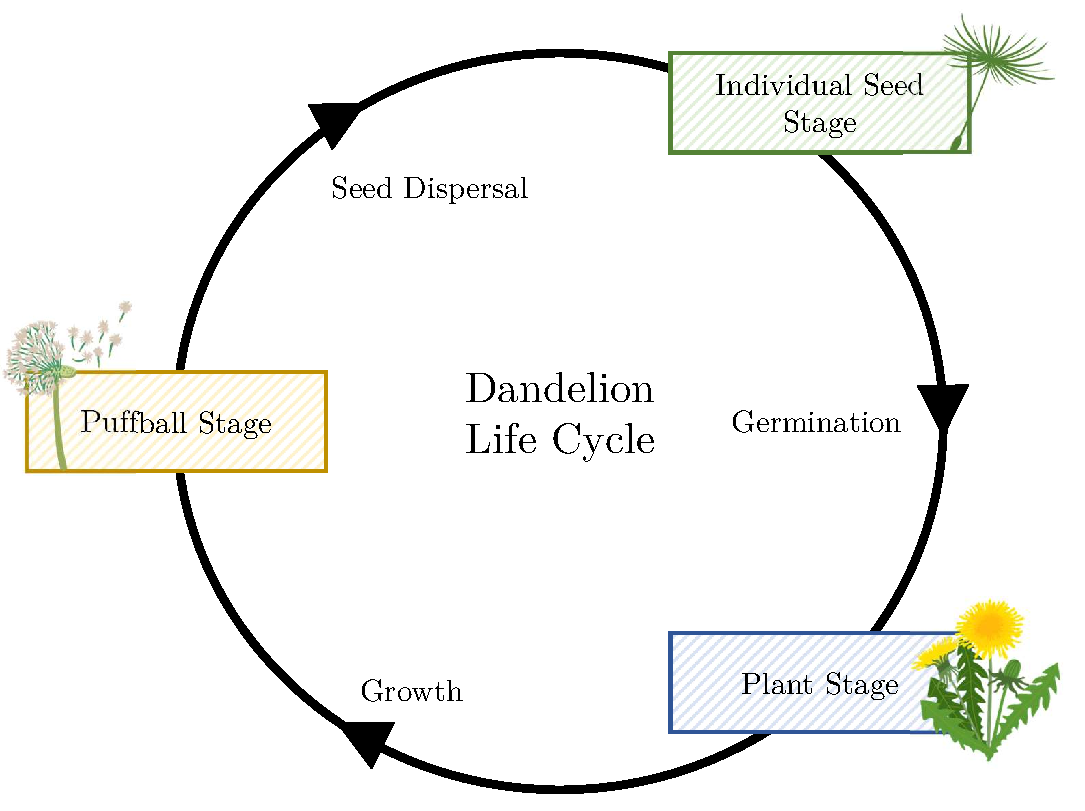
\includegraphics[scale=0.5]{figures/dandelionlifecycle.pdf}
    \captionsetup{width=0.9\textwidth}
    \caption{\textbf{Dandelion life-cycle.} A recurring process from seed to germination to growth, then the dispersal of seeds again.}
    \label{fig:dandelionlifecycle}
\end{figure}

\subsubsection{Phase 1: Seed}
Dandelion seeds begin their dispersal process from a puffball. However, only around 2-4\% of the many seeds make it past the initial dispersal stage, the remainder of which is lost to consumers \cite{noauthor_dandelion_nodate-2}. Upon landing, it will lay dormant until it meets certain environmental conditions to germinate and begin its plant growth process. 

% In order for a seed to grow, certain environmental conditions must be met. In the event that conditions are not met, seeds often enter a dormant stage where they can remain beneath the earth until environmental conditions are met. Unlike most plants, the dandelion seed cannot lay dormant for long due to the high likelihood of premature consumption \cite{noauthor_dandelion_nodate-2} Of the small amount that does survive, they typically germinate right away and survive until the next season \cite{noauthor_dandelion_nodate-2}.

\subsubsection{Phase 2: Plant}
Next, the seed continues into the plant growth process. Here, certain environmental conditions, such as the right temperature, light, and nutrients in the soil can aid the growth of a dandelion. The dandelion is no longer considered growing when it has reached its puffball phase.

\subsubsection{Phase 3: Puffball}
The puffball stage occurs when the white seeds of the plant fully emerge, replacing the distinctive yellow flowers  \cite{board_of_pesticides_control_maine_dacf_dandelion-taraxacum_nodate}. Once ready, the dandelion releases its seeds to the power of the wind which scatters the seeds into an everlasting journey.

\subsubsection{Death}
As a perennial plant, the taproot of the dandelion allows the plant to keep its roots for another year while the flowers and stem wither away in the winter. In the event of any damage to the portion of the plant above ground, the taproot remains rooted, and so, the dandelion continues to survive \cite{farmshowGrowingDandelions}. For a dandelion to die fully, either the taproot is entirely removed from the ground, or the plant reaches its life expectancy of 10-13 years \cite{noauthor_garden_nodate}. In Figure~\ref{fig:dandelionlifecycle}, we summarize the life cycle of a dandelion (from seed to puffball), from which we draw inspiration for our dandelion spread model.

\subsection{Problem Restatement}

 \begin{enumerate}
 \item Develop a model to represent the spread of dandelions over the course of 1, 2, 3, 6 and 12 months, given the model begins with a single dandelion in its puffball stage adjacent to an open, one-hectare plot of land.
\item Formulate a mathematical model to determine an "impact factor" for invasive species.
\subitem a. Compute an impact factor for dandelions to test the model.
\subitem b. Determine the impact factor for two other non-native plant species of 
our choice that are often considered invasive.

\end{enumerate}
